% The underlying theory of the report

\subsection{One digital pixel} \label{sec:oneDigitalPixel}


Each pixel in the camera is constructed as shown in figure~\ref{fig:pixelschematic}.
The photo diodes detecting the actual light does, in many ways, act as a current source dependent on the light on it, when a picture is taken this
current is let through M1 and used to charge CS.
Before each picture is taken, the transistor M2 is opened to reset the voltage stored over the capacitor CS.

It is important that the transistors M1 and M2 are not let on simultaneously for extended periods of time as this results in a short circuit from VDD to VSS thorugh PD1.
While the photo diode limits the current, this still might lead to excessive power usage and subsequent heating issues over time.


\begin{figure}[htbp]
  \centering
  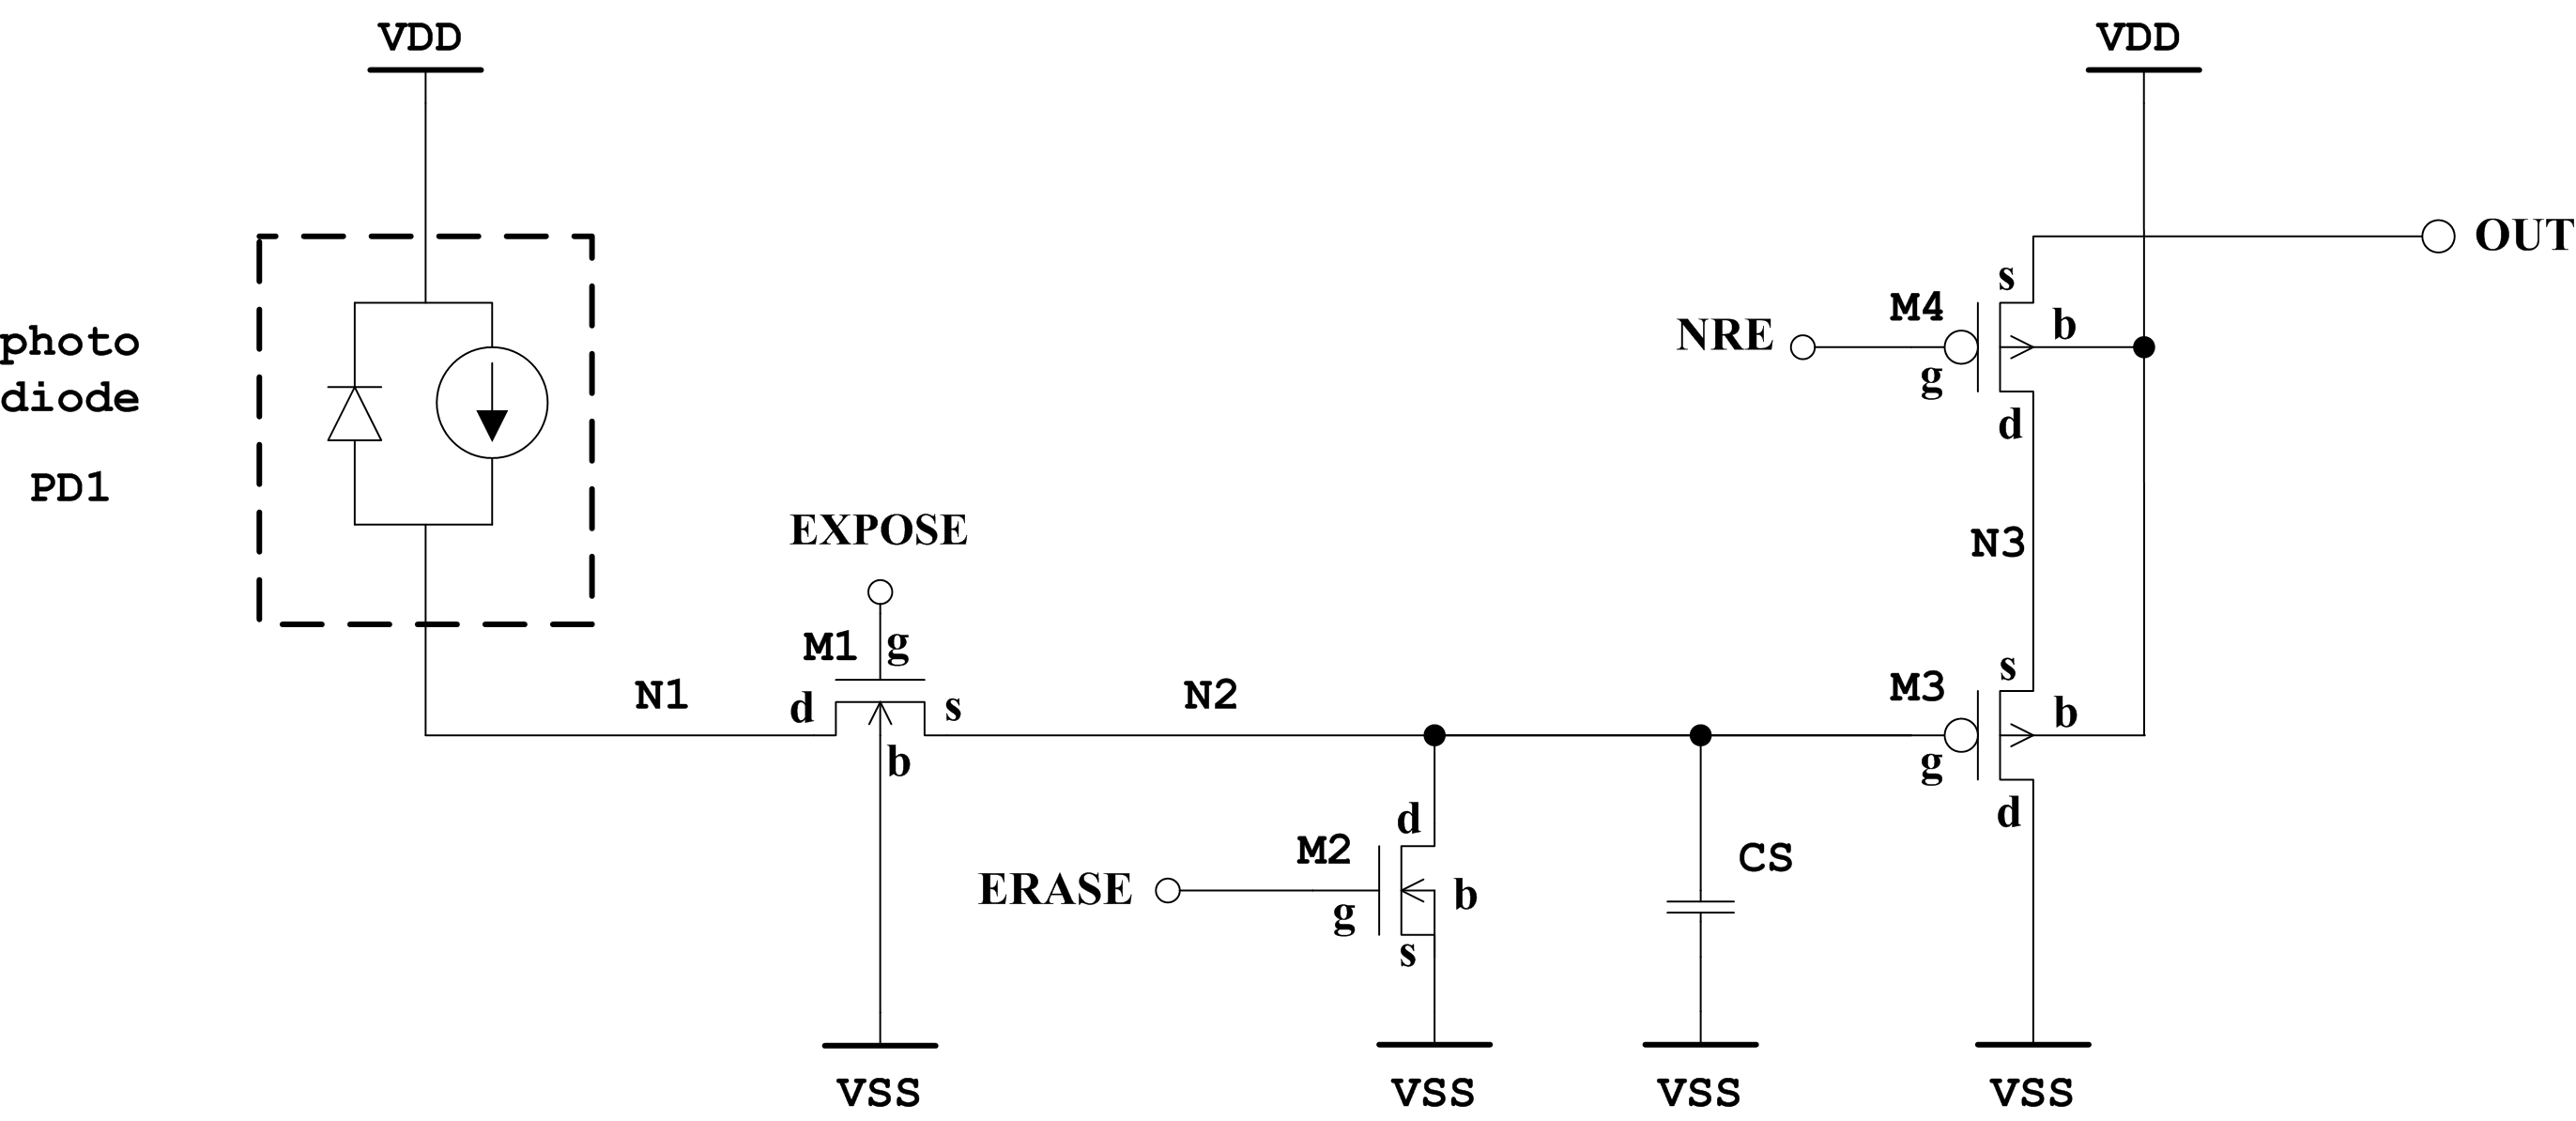
\includegraphics[width=0.85\textwidth]{figures/pixel}
  \caption{Schematic of one pixel with readout circuit, figure from~\cite{oppgave}}\label{fig:pixelschematic}
\end{figure}


The transistor M3 is used to convert the voltage stored over CS into a variable resistance between the nodes N3 and VSS for a nondestructive readout of the pixel,
the transistor M4 functions as a simple switch to isolate the pixel from OUT to free the wire when other pixels in the camera are using it.


\subsection{Leakage through transistors} \label{sec:leakagecurrent}

We will in this project assume that all voltage transient are so slow that no leakage current is present between gate and the other ports of any of the transistors,
in the same way we assume there are no leakage currents through any of the capacitors.

As described in Analog~integrated~circuit~design~\cite{AnalogBook} the current from drain to source $I_D \propto \frac{W}{L}$.
This also makes sense from a geometric point of view.

In order to minimize the leakage current through a transistor that is shut off $\frac{W}{L}$ should be minimized.

\subsection{Conceptual workings of a camera controller}

As shown in figure~\ref{fig:analogCamera} found in Appendix~\ref{ap:Schematics} the behavior of the pixels depend on several digital input signals,
the job of the camera controller is therefore to trigger these in the desired order.
The requirements to be met by the controller are as follows:

\begin{itemize}
\item Pull the erase pin high except when exposing or reading the image
\item Pull the expose pin high for an appropriate length of time as defined by the user
\item Read out the values of all pixels in the correct order avoiding interference between different pixels on the same ADC.
\item Enable the user to reset the whole system. Though the image being taken might be lost the camera should function normally afterwards.
\end{itemize}
